\chapter{Analysis and design of the access management system} In this chapter I will describe the access management system designed for the new Bi-DBS portal frontend, based on roles and permissions analysis. The goal is to simplify the access management system if it is possible and provide an overview of the permissions for existing roles.


\section{Roles} The BI-DBS portal receives information about an authorized user from the study information system(KOS) based on the course information. The course information contains the identifier of the semester and the type of study program. Generally, there are eight user roles that are defined by the KOS for subjects and courses.\\

\noindent \textbf{Base roles for subjects and their general description:}

\begin{itemize}
    \item \emph{Teacher.} 
    \item \emph{Student.} 
\end{itemize}

\noindent \textbf{Teacher roles for subjects and their general description:}

\begin{itemize}
    \item \emph{Guarantor.} Guarantor is a course administrator. Thus a person with this role typically have all permissions across all course management.
    \item \emph{Examiner.} Examiners are responsible for managing and estimating students exams. Therefore, this role would usually provide an access to exam materials and students grades view and management.
    \item \emph{Editor.} Editor is person who can edit the information about the subject.
    \item \emph{Lecturer.} 
    \item \emph{Instructor.} 
    \item \emph{Laboratory instructor.}
\end{itemize}

% https://kosapi.fit.cvut.cz/projects/kosapi/wiki/Course
According to the BI-DBS subject ... roles like laboratory instructor and editor are no

\noindent From these six roles in fact. Based on the feedback from the teachers and developers of the current BI-DBS portal and my own research, we came to the conclusion that the access management system can be simplified by grouping the roles into three hierarchical layers.\\

Beginning with a student role. All instructors, lectors, examiners, and also guarantors need to have an overview of how the whole application works including the students side to be able to explain how to work with the portal, as well as they can use it for teaching. Therefore all the roles should have permission to access students 



\begin{figure}[h]
\centering
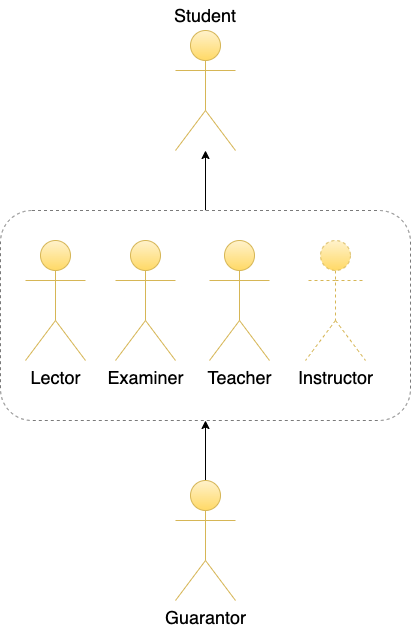
\includegraphics[scale=0.57]{../png/role.png}
\caption{Roles hierarchy}\label{picture:roles}
\end{figure}

\newpage
\section{Permissions} modules and permissions... example of 
 diagram of 


modules
\begin{itemize}
    \item Administration
    \item Semester Work
    \item Tests
    \item Connections
    \item Students score
    \item Users
\end{itemize}